\section[Proof Discharge Algorithm]{Proof Discharge Algorithm through Illustative Examples}
\label{sec:examples}
This section demonstrates our proof discharge algorithm through examples.
We consider proof obligations generated due to invariants shown in \cref{tab:llproductInv,fig:llTraverseProductInv}
for the product-CFGs in \cref{fig:llAllocProductCFG,fig:llTraverseProduct} respectively.
We start by describing the properties of the proof discharge algorthm.
We also list the properties of the proof obligations generated by our equivalence checker;
these properties are essential for the correctness of our proof discharge algorithm.
Next, the proof discharge algorithm is explored using sample proof obligations,
and we finish with a pseudo-code of the algorithm.

\subsection{Properties of Proof Discharge Algorithm}
\label{sec:proofalgoprops}
An algorithm that evaluates the truth value of a proof obligation is called a
{\em proof discharge algorithm}.
In case a proof discharge algorithm deems a proof obligation to be unprovable,
it is expected to return {\em false} with a set of counterexamples that falsify
the proof obligation.
A proof discharge algorithm is {\em precise} if for all proof obligations,
the truth value evaluated by the algorithm is identical to the proof obligation's
{\em actual} truth value.
A proof discharge algorithm is {\em sound} if:
(a) whenever it evaluates a proof obligation to true,
the actual truth value of that proof obligation is also true,
and (b) whenever it generates a counterexample, that counterexample
must falsify the proof obligation.
However, it is possible for a sound proof discharge algorithm to return false
(without counterexamples) when the proof obligation was actually provable.

For proof obligations generated by our equivalence checker procedure,
it is always safe for a proof discharge algorithm to return false (without counterexamples).
Keeping this in mind, our proof discharge algorithm is designed to be {\em sound}.
Conservatively evaluating a proof obligation to false (when it was actually provable)
may prevent the equivalence proof from completing successfully.
However, importantly, the overall equivalence procedure remains sound i.e.
(a) either it successfully finds a valid proof of equivalence (bisimulation relation)
or (b) it conservatively returns {\em unknown}.

Resolving the truth value of a proof obligation that contains a \recursiveRelation{}
such as $\sv{l} \indEq{} \lifted{list}{\mem{}}{lnode}{\cv{l}}$ is unclear.
Fortunately, the shapes of the proof obligations generated by our equivalence
checker are restricted.
Our equivalence checking algorithm ensures that, for an invariant
$\phi_s=({\tt \phi^{1}_s \land \phi^{2}_s \land ... \land \phi^{k}_s})$,
at any node $s$ of a product-CFG,
if a \recursiveRelation{} appears in $\phi_s$, it
must be one of $\phi^{1}_s$, $\phi^{2}_s$, ..., or $\phi^{k}_s$. We call
this the {\em conjunctive \recursiveRelation{}} property of an invariant $\phi_s$.

A proof obligation
$\hoareTriple{\phi_s}{e}{\phi_d}$, where $e=(\rho_S,\rho_C)$,
gets lowered using
${\tt WP}_{e}(\phi_d)$ (as shown in \cref{eqn:firstOrderFormula}) to a first-order logic formula of the following form:

\begin{equation}
\label{eqn:proofObligationShape}
(\eta^{l}_1 \land \eta^{l}_2 \land ... \land \eta^{l}_m) \Rightarrow (\eta^{r}_1 \land \eta^{r}_2 \land ... \land \eta^{r}_n)
\end{equation}

Thus, due to the conjunctive \recursiveRelation{} property of $\phi_s$ and $\phi_d$, any
\recursiveRelation{} in \cref{eqn:proofObligationShape} must appear as
one of $\eta^{l}_i$ or $\eta^{r}_j$.
To simplify proof obligation discharge,
we break a first-order logic proof obligation $P$ of the form in \cref{eqn:proofObligationShape}
into multiple smaller proof obligations
of the form
$P_j:(\lhs{} \Rightarrow{\tt \eta^{r}_j})$, for $j=1..n$. Each proof obligation
$P_j$ is then discharged separately.  We call this conversion from
a bigger query to multiple smaller queries, {\em \rhs{}-breaking}.

We provide a sound (but imprecise) proof discharge algorithm that converts
a proof obligation generated by our equivalence checker into a series
of SMT queries.
Our algorithm begins by categorizing a proof obligation into
one of three types; each type is discussed separately in subsequent
sections.
The categorization is based on a specialized unification procedure, which we describe next.

\subsection{Iterative Unification and Rewriting Procedure}
\label{sec:unifyandrewrite}
We begin with some definitions.
An expression $e$ whose top-level constructor is a lifting
constructor, e.g., $e=\lifted{list}{\mem{}}{lnode}{\cv{l}}$,
is called a {\em lifted expression}.
An expression $e$ of the form \prodAccess{v}{a_1,a_2,.,a_n} i.e.
a variable with {\em zero} or more {\em accessor}-operators applied on it,
is called a {\em pseudo-variable}.
Note that, a variable $v$ is a pseudo-variable.
An expression $e$ in which (a) all accessors (e.g., `\prodAccess{\_}{tail}') appear
in a pseudo-variable, and (b) each {\em is}-operator (e.g., `\sumIs{\_}{LCons}') operate
on a pseudo-variable, is called a {\em canonical expression}.
It is possible to convert any expression $e$ into its canonical form $\hat{e}$.
For example, the canonical form of $a + \prodAccess{\cons{LCons}(b,l)}{tail,val}$
is given by $a + \prodAccess{l}{val}$, where \prodAccess{l}{val} is a pseudo-variable.

Consider the expression tree of a canonical expression $\hat{e}$.
The internal nodes of $\hat{e}$ represents ADT data constructors and
the \sumDtor{} sum-deconstruction operator.
The leaves of $\hat{e}$ (also called {\em atoms} of $\hat{e}$) are the
pseudo-variables (of scalar and ADT type),
the scalar expressions (of \type{unit}, \type{bool} and \type{i<N>} types),
and lifted expressions.

The {\em expression path} to a node $v$ in $\hat{e}$'s tree is the path from the root
of $\hat{e}$ to the node $v$.
The {\em expression path condition} represents the conjunction of all the \underline{\tt if}
conditions (if the \underline{\tt then} branch of taken along the path), or their
negation (if the \underline{\tt else} branch is taken along the path) for each \sumDtor{}
along the path.
For example, in the expression \sumIf{c} \sumThen{a} \sumElse{b},
the expression path condition of $c$ is {\tt true}, of $a$ is $c$,
and of $b$ is $\neg c$.

When we attempt to unify two expressions,
we unify their tree structures created by data constructors and the \sumDtor{} operator.
The unification procedure either fails to unify, or it returns tuples \corrtuple{p_1}{a_1}{p_2}{e_2} where atom $a_1$
at expression path condition $p_1$ in one expression is correlated
with expression $e_2$ at expression path condition $p_2$ in the other expression.

For two non-atomic expressions, $e_1$ and $e_2$ to unify successfully,
it must be true that either the top-level operator in $e_1$ and $e_2$ is
the same data constructor (in which case an unification is attempted for each
of their children), {\em or} the top-level operator in atleast one of $e_1$ or $e_2$ is \sumDtor{}.

If the top-level operator in {\em exactly one} of $e_1$ and $e_2$ (say $e_2$) is \sumDtor{},
then $e_1$ must have a data constructor at its root.
Given $e_2 = $ \sumIf{c} \sumThen{e_2^{\tt th}} \sumElse{e_2^{\tt el}},
we first attempt to unify $e_1$ with the \underline{if} branch $e_2^{\tt th}$ --- if unification succeeds,
we also unify $c$ (\underline{then} condition) with {\em true}.
Otherwise, we unify $e_1$ with the \underline{else} branch $e_2^{\tt el}$ and $\neg c$ (\underline{else} condition) with {\em true}.

If the top-level operator in both $e_1$ and $e_2$ is \sumDtor{},
we unify each child (condition and branch expressions) of the corresponding
\sumDtor{} operators.
Recall that the \sumDtor{} operator (introduced in \cref{sec:ir}) for an ADT $T$ must have exactly one branch
for each data constructor of $T$, and the branch associated with the data constructor $V$
has $V$ in its top-level.
Whenever we descend down an \sumDtor{} operator, we conjunct the \underline{\tt if} condition (if \underline{\tt then} branch is taken)
or its negation (if \underline{\tt else} branch is taken) with its associated expression path condition.
This allows us to keep track of the expression path conditions for both expressions
during recursive descent to their children.

If one of $e_1$ and $e_2$ (say $e_2$) is atomic,
unification always succeeds and returns \corrtuple{p_2}{e_2}{p_1}{e_1}.
With each atom of an ADT type, we associate an {\em unrolling procedure}.
By definition, an ADT atom is either a pseudo-variable or a lifted expression.
Each (pseudo-)variable is associated with its unrolling procedure governed by its type.
For example, the unrolling procedure for a \type{List} variable $l$ is given by $U_S$ (\cref{eqn:specDeconstruct}).
For lifted expressions, the unrolling procedure is given by its definition, e.g., $U_C$ (\cref{eqn:clist})
for the lifting constructor \lift{list}{\mem{}}{lnode}.

Given two {\em canonical} expressions $e_a$ and $e_b$ at expression path conditions $p_a$ and $p_b$
respectively, an {\em iterative unification and rewriting procedure}
$\Theta(p_a,e_a,p_b,e_b)$ is used to identify a set of correlation tuples
between the atoms in the two expressions.
This iterative procedure begins with an attempt to unify $e_a$ and $e_b$.
If this unification fails, we return a failure for the original expressions $e_a$ and $e_b$.
Else, we obtain correlation tuples between atoms and expressions
(with their expression path conditions).
If the unification correlates an atom $a_1$ at expression path condition $p_1$
with another atom $a_2$ at expression path condition $p_2$, we add \corrtuple{p_1}{a_1}{p_2}{a_2} to the final output.
Otherwise, if the unification correlates an atom $a_1$ at expression path condition $p_1$
to a non-atomic expression $e_2$ at expression path condition $p_2$,
we {\em rewrite} $a_1$ using its unrolling procedure to obtain expression $e_1$.
The unification algorithm then proceeds by unifying $e_1$ and $e_2$ through
a recursive call to $\Theta(p_1,e_1,p_2,e_2)$.
The maximum number of rewrites performed by $\Theta(p_a,e_a,p_b,e_b)$ (before termination)
is bounded by the sum of number of ADT data constructors in $e_a$ and $e_b$.
The algorithms responsible for canonicalization, unification, and iterative unification and rewriting
are further discussed in \cref{sec:canonicalalgo,sec:unifalgo,sec:unifyandrewritealgo} respectively.

For a \recursiveRelation{} $l_1 \indEq{} l_2$, we unify (canonicalized) $l_1$ and $l_2$ through a
call to $\Theta(true,l_1,true,l_2)$.
If the $n$ tuples obtained after a successful unification are \corrtuple{p_1^i}{a_1^i}{p_2^i}{a_2^i}
(for $i=1\ldots n$), then the {\em decomposition} of $l_1 \indEq{} l_2$ is defined as:

\begin{equation}
\label{eqn:decompose}
l_1 \indEq{} l_2 \Leftrightarrow \bigwedge \limits_{i=1}^n (p_1^i \land p_2^i \rightarrow (a_1^i = a_2^i))
\end{equation}

For example, the unification of `\sumIf{c_1} \sumThen{\cons{LNil}} \sumElse{\cons{LCons}(0,l_1)}'
and `\sumIf{c_2} \sumThen{\cons{LNil}} \sumElse{\cons{LCons}(i, \lifted{list}{\mem{}}{lnode}{l_2})}'
yields the correlation tuples: $(true,true,c_1,c_2)$, $(\neg c_1, \neg c_2, 0, i)$ and
$(\neg c_1, \neg c_2, l_1, \lifted{list}{\mem{}}{lnode}{l_2})$.
Consequently, the \recursiveRelation{} ``\sumIf{c_1} \sumThen{\cons{LNil}} \sumElse{\cons{LCons}(0,l_1)} \indEq{}
\sumIf{c_2} \sumThen{\cons{LNil}} \sumElse{\cons{LCons}(i, \lifted{list}{\mem{}}{lnode}{l_2})}''
decomposes into $(c_1 = c_2) \land (\neg c_1 \land \neg c_2 \rightarrow 0 = i)
\land (\neg c_1 \land \neg c_2 \rightarrow l_1 \indEq{} \lifted{list}{\mem{}}{lnode}{l_2})$.
Similarly, the decomposition of $l_1 \indEq{} \cons{LCons}(42, \lifted{list}{\mem{}}{lnode}{l_2})$ is given by
$(\sumIs{l_1}{LCons}) \land (\sumIs{l_1}{LCons} \rightarrow \prodAccess{l_1}{val}=42)
\land (\sumIs{l_1}{LCons} \rightarrow \prodAccess{l_1}{next} \indEq{} \lifted{list}{\mem{}}{lnode}{l_2})$
\footnote{(\sumIs{l_1}{LCons}) is equivalent to $\neg (\sumIs{l_1}{LNil}$).
In general, for an ADT value $v$ of type $T$ (with data constructors $V_{\tt 1}, V_{\tt 2}, \dots, V_{\tt k}$),
exactly one of (\sumIs{v}{\mathnormal{V}_{\tt i}}) is true.}.
In case of a failed unification, the {\em decomposition} is defined to be {\em false},
e.g., $\cons{LNil} \indEq{} \cons{LCons}(0, l)$ decomposes into $false$.

Each conjunctive clause of the form $(p_1^i \land p_2^i \rightarrow (a_1^i = a_2^i))$\footnote{
If $a_1^i$ and $a_2^i$ are ADT values, then we replace $a_1^i = a_2^i$ with $a_1^i \indEq{} a_2^i$.}
in the decomposition is called a {\em decomposition clause}.
A decomposition clause may relate only atomic values, i.e.,
it may relate (a) two scalars or (b) two ADT variable(s) and/or lifted expression(s).
However, we restrict the shapes of \recursiveRelation{} invariants such that each
\recursiveRelation{} in its decomposition {\em strictly} relates ADT values to lifted expressions.
The invariant shapes along with the invariant inference procedure is discussed in \cref{sec:invinferalgo}.
We {\em decompose} a \recursiveRelation{} by replacing it with its decomposition.
We {\em decompose} a proof obligation by decomposing all \recursiveRelations{} in it.

\subsection{Categorization of Proof Obligations}
We {\em unroll a \recursiveRelation{} $l_1 \indEq{} l_2$} by rewriting the
top-level expressions $l_1$ and $l_2$ through their unrolling procedures (if possible)
and decomposing it.
We {\em unroll an expression $e$} by unrolling each \recursiveRelation{} in $e$.
More generally, the $k$-unrolling of $e$ is found by unrolling the $(k-1)$-unrolling
of $e$ recursively.
For a decomposed proof obligation $P_D:\lhs{} \Rightarrow \rhs{}$, we identify its $k$-unrolling (say $P_K$),
where $k$ is a fixed parameter called the {\em unrolling parameter}.
After $k$-unrolling, we {\em eliminate} those decomposition clauses $(p_1 \land p_2 \rightarrow (a_1 = a_2))$
in $P_K$ whose $(p_1 \land p_2)$ evaluates to false under \lhs{} ignoring all \recursiveRelations{},
yielding an equivalent proof obligation, say $P_E$.
For example, the one-unrolling of $P: \lhs{} \Rightarrow l \indEq{} \lifted{list}{\mem{}}{lnode}{0}$,
after elimination, yields $P_E: \lhs{} \Rightarrow \sumIs{l}{LNil}$.
We categorize a proof obligation $P: \lhs{} \Rightarrow \rhs{}$ based on the $k$-unrolled form
of its decomposition (i.e. $P_E$) as follows:

\begin{itemize}
\item Type I: $P_E$ does not contain \recursiveRelations{}
\item Type II: $P_E$ contains \recursiveRelations{} {\em only} in the \lhs{}
\item Type III: $P_E$ contains \recursiveRelations{} in the \rhs{}
\end{itemize}

The categorization method is {\em sound} as long as the elimination of decomposition
clauses is sound (but possibly not precise).
In other words, it is possible that we are unable to eliminate a \recursiveRelation{} in $P_K$,
due to an imprecise algorithm for elimination of decomposition clauses.
However, our proof discharge algorithm remains sound irrespective of such imprecision
during categorization.
Henceforth, we will simply use $k$-unrolling of $P$ to refer to $P_E$ directly.
Next, we describe the algorithm for each type of proof obligations
in \cref{sec:cat1,sec:cat2,sec:cat3}.

\subsection{Handling Type I Proof Obligations}
\label{sec:cat1}
In \cref{fig:llAllocProductCFG}, consider a proof obligation generated
across the product-CFG edge \scedge{0}{0}{3}{3}
while checking if the {\circled{\footnotesize I4}} invariant in \cref{tab:llproductInv},
$\sv{l} \indEq{} \lifted{list}{\mem{}}{lnode}{\cv{l}}$ holds at (\scpc{3}{3}):
\hoareTriple{\scpcinv{0}{0}}{\spath{0,3},\cpath{0,3}}{\sv{l} \indEq{} \lifted{list}{\mem{}}{lnode}{\cv{l}}}.
The precondition $\scpcinv{0}{0} \equiv (\sv{n} = \cv{n})$ does not contain a \recursiveRelation{}.
When lowered to first-order logic through {\tt WP}$_{\spath{0,3},\cpath{0,3}}$, this translates to
$\sv{n} = \cv{n} \Rightarrow \cons{LNil} \indEq{} \lifted{list}{\mem{}}{lnode}{0}$.
Here, \cons{LNil} is obtained for \sv{l} and {\tt 0} (null) is obtained for \cv{l}.
The one-unrolled form of this proof obligation yields
$\sv{n} = \cv{n} \Rightarrow true$ which trivially resolves to true.

Consider the following example of a proof obligation:
\hoareTriple{\scpcinv{0}{0}}{\spath{0,3,5,3},\cpath{0,3}}{\sv{l} \indEq{} \lifted{list}{\mem{}}{lnode}{\cv{l}}}.
Notice, we have changed the path in \sprog{} (with CFG \cref{fig:llAllocSpecIRCFG}) to \spath{0,3,5,3} here.
In this case, the corresponding first-order logic formula evaluates to:
$(\sv{n} = \cv{n}) \land (0 <_u \sv{n}) \Rightarrow \cons{LCons}(0, \cons{LNil}) \indEq{} \lifted{list}{\mem{}}{lnode}{0}$,
where $(0 <_u \sv{n})$ is the path condition for the path \spath{0,3,5,3}.
One-unrolling of this proof obligation decomposes \rhs{} into false due to
failed unification of \cons{LCons} and \cons{LNil}.
The proof obligation is further discharged using an SMT solver
which provides a counterexample (model) that evaluates the
formula to false. For example, the counterexample $\{ \mapping{\sv{n}}{42}, \mapping{\cv{n}}{42} \}$
evaluates this formula to false.
These counterexamples assist in faster convergence of our correlation search and invariant inference procedures
(as we will discuss later in \cref{sec:searchalgo,sec:invinferalgo}).

Thus for type I queries, $k$-unrolling reduces all (if any) \recursiveRelations{}
in the original proof obligation into scalar equalities.
The resulting query is further discharged using an SMT solver.
\Cref{sec:proofalgo} contains a deeper analysis of the following aspects of our proof discharge algorithm:
(a) translation of formula to SMT logic (\cref{sec:smtencoding}), and
(b) reconstruction of counterexamples from models returned by the SMT solver (\cref{sec:cerecons}).
Assuming a capable enough SMT solver,
all proof obligations in type I can be discharged precisely, i.e., we can always
decide whether the proof obligation evaluates to true or false.
If it evaluates to false, we also obtain counterexamples.

\subsection{Handling Type II Proof Obligations}
\label{sec:cat2}
Consider the proof obligation for \circled{\small I2} invariant $\sv{sum} = \cv{sum}$
across edge \scedge{2}{2}{2}{2} in \cref{fig:llTraverseProduct}:
\hoareTriple{\scpcinv{2}{2}}{\spath{2,5,2}, \cpath{2,4,2}}{\sv{sum} = \cv{sum}}, where
the node invariant \scpcinv{2}{2} contains the \recursiveRelation{} $\sv{l} \indEq{} \lifted{list}{\mem{}}{lnode}{\cv{l}}$.
The corresponding (simplified) first-order logic formula for this proof obligation is:
$\sv{l} \indEq \lifted{list}{\mem{}}{lnode}{\cv{l}} \land (\sv{sum} = \cv{sum}) \land (\sumIs{\sv{l}}{LCons}) \land (\cv{l}\neq0) \Rightarrow (\sv{sum} + \prodAccess{\sv{l}}{val}) = (\cv{sum} + \structPointer{\cv{l}}{\mem{}}{lnode}{val})$.
We fail to remove the \recursiveRelation{} on the \lhs{} even after
$k$-unrolling for any finite unrolling parameter $k$ because both sides of \indEq{}
represent list values of arbitrary length.
In such a scenario, we do not know of an efficient
SMT encoding for the \recursiveRelation{} $\sv{l} \indEq{} \lifted{list}{\mem{}}{lnode}{\cv{l}}$.
Ignoring this \recursiveRelation{} will incorrectly (although soundly) evaluate
the proof obligation to false; however, for a successful equivalence
proof, we need the proof discharge algorithm to evaluate it to true. Let's call this
requirement \circled{\footnotesize R1}.

Now, consider the proof obligation formed by correlating two iterations
of the loop in program \sprog{} (with CFG \cref{fig:llTraverseSpecCFG}) with
one iteration of the loop in program \cprog{} (with CFG \cref{fig:llTraverseCCFG}):
\hoareTriple{\scpcinv{2}{2}}{\spath{2,5,2,5,2}, \cpath{2,4,2}}{\sv{sum} = \cv{sum}}.
The equivalent first-order logic formula is:
$\sv{l} \indEq{} \lifted{list}{\mem{}}{lnode}{\cv{l}} \land (\sv{sum} = \cv{sum}) \land (\sumIs{\sv{l}}{LCons}) \land (\sumIs{\prodAccess{\sv{l}}{tail}}{LCons}) \Rightarrow (\sv{sum} + \prodAccess{\sv{l}}{val} + \prodAccess{\sv{l}}{tail,val}) = (\cv{sum} + \structPointer{\cv{l}}{\mem{}}{lnode}{val})$.
Similar to the prior proof obligation, its equivalent first-order logic formula contains a \recursiveRelation{} in the \lhs{}.
Clearly, this proof obligation should evaluate to false.
Whenever a proof obligation evaluates to false, we
expect an ideal proof discharge algorithm to generate
counterexamples that falsify the proof obligation.
Let's call this requirement \circled{\footnotesize R2}.
Recall that these counterexamples help in faster
convergence of our correlation search and invariant inference procedures.

To tackle requirements \circled{\footnotesize R1} and \circled{\footnotesize R2},
our proof discharge algorithm converts the original proof obligation $P: \hoareTriple{\phi_s}{e}{\phi_d}$
into two approximated proof obligations $(P_{pre-o}: \hoareTriple{\phi^{o_{d_1}}_s}{e}{\phi_d})$
and $(P_{pre-u}: \hoareTriple{\phi^{u_{d_2}}_s}{e}{\phi_d})$.
Here $\phi^{o_{d_1}}_s$ and $\phi^{u_{d_2}}_s$ represent the over- and under-approximated
versions of precondition $\phi_s$ respectively, and $d_1$ and $d_2$ represent
{\em depth parameters} that indicate the degree of over- and under-approximation.
To explain our over- and under-approximation scheme, we
first introduce the notion of {\em depth of an ADT value}.

\subsubsection{Depth of ADT Values}
\label{sec:adtdepth}
To define depth of an ADT value $v$, we view the value as a tree $\mathcal{T}(v)$.
The internal nodes of $\mathcal{T}(v)$ represent ADT data constructors and
the leafs (also called {\em terminals}) represent scalar values (e.g. bitvector literals).
The depth of a data constructor or a scalar in $v$ is simply the depth of
its associated node in $\mathcal{T}(v)$.
The {\em depth} of ADT value $v$ is defined as the depth of $\mathcal{T}(v)$.
For example, the depth of $\cons{LCons}(1, \cons{LCons}(4, \cons{LNil}))$ is {\tt 2}.
\Cref{fig:exprtrees} shows the tree representation and depths for multiple ADT values.

\begin{figure}
\begin{tabular}{@{}c@{}c@{}c@{}}
\begin{subfigure}[b]{0.32\textwidth}
\begin{center}
{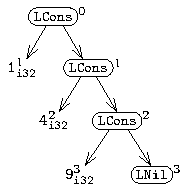
\includegraphics[scale=1.3]{chapters/figures/figExprtreeList1.pdf}}
\end{center}
\caption{\label{fig:exprtreelist}\type{List} = \cons{LNil} | \newline \cons{LCons}(\type{i32}, \type{List})}
\end{subfigure}%
&
\begin{subfigure}[b]{0.28\textwidth}
\begin{center}
{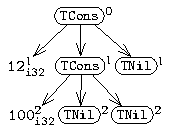
\includegraphics[scale=1.3]{chapters/figures/figExprtreeTree1.pdf}}
\end{center}
\vspace{18px}
\caption{\label{fig:exprtreetree}\type{Tree} = \cons{TNil} | \newline \cons{TCons}(\type{i32}, \type{Tree}, \type{Tree})}
\end{subfigure}%
&
\begin{subfigure}[b]{0.4\textwidth}
\begin{center}
{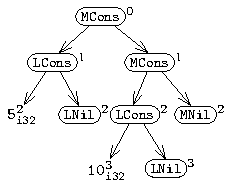
\includegraphics[scale=1.3]{chapters/figures/figExprtreeMatrix2.pdf}}
\end{center}
\caption{\label{fig:exprtreematrix}\type{Matrix} = \cons{MNil} | \newline \cons{MCons}(\type{List}, \type{Matrix})}
\end{subfigure}%
\\
\end{tabular}
\caption{\label{fig:exprtrees}Tree representation of three values, each of type \type{List}, \type{Tree} and \type{Matrix} respectively. The depths are shown as superscripts for each node in the trees.}
\end{figure}


\subsubsection{Overapproximation and Underapproximation of Recursive Relations}
\label{sec:approxdefs}
The $d$-depth overapproximation of a \recursiveRelation{} $l_1 \indEq{} l_2$,
denoted by $l_1 \indEqDepth{d} l_2$, represents the condition that
$l_1$ and $l_2$ are {\em recursively equal up to depth $d$}. i.e.,
$l_1$ and $l_2$ have identical structures and all
{\em terminals} at depths $\leq d$ in the trees of both values
are equal (under the precondition that the terminals exist);
however, terminals at depths $>d$ may have different values.
$l_1 \indEqDepth{d} l_2$ (for finite $d$) is a weaker
condition than $l_1 \indEq{} l_2$ (i.e. overapproximation).
The true equality i.e. $l_1 \indEq{} l_2$ can be thought of as equality of structures
and all terminals up to an unbounded depth i.e. $l_1 \indEqDepth{\infty} l_2$.

The $d$-depth underapproximation of a \recursiveRelation{} $l_1 \indEq{} l_2$
is written as $l_1 \indEqUapprox{d} l_2$, where $\indEqUapprox{d}$ represents
the condition that $l_1$ and $l_2$ are {\em recursively equal and bounded to depth $d$},
i.e., $l_1$ and $l_2$ have a maximum depth $\leq d$ {\em and}
they are recursively equal up to depth $d$.
Thus, $l_1 \indEqUapprox{d} l_2$ is equivalent to
$\depthBound{d}{l_1} \land \depthBound{d}{l_2} \land l_1 \indEqDepth{d} l_2$,
where $\depthBound{d}{l}$ represents the condition that the maximum
depth of $l$ is $d$.
$l_1 \indEqUapprox{d} l_2$ (for finite $d$) is a stronger condition than
$l_1\indEq{}l_2$ (i.e. underapproximation)
as it bounds the depth to $d$ while also ensuring equality till depth $d$.
For arbitrary depths $a$ and $b$ ($a \leq b$),
the approximations of $l_1 \indEq{} l_2$ are related as follows:

\begin{equation}
\label{eqn:approxrels}
l_1 \indEqUapprox{a} l_2 \Rightarrow l_1 \indEqUapprox{b} l_2 \Rightarrow l_1 \indEq{} l_2 \Rightarrow l_1 \indEqDepth{b} l_2 \Rightarrow l_1 \indEqDepth{a} l_2
\end{equation}

\subsubsection{Reduction of Approximate Recursive Relations}
\label{sec:approxdecomp}
Unlike the original \recursiveRelation{} $l_1 \indEq{} l_2$,
its approximations $l_1\indEqDepth{d}l_2$ and $l_1\indEqUapprox{d}l_2$ can be reduced into
equivalent conditions absent of \recursiveRelations{}.
Hence, these approximations can be encoded and subsequently discharged by a SMT solver.

\begin{itemize}
\item $l_1 \indEqDepth{d} l_2$ is equivalent to the condition that
the tree structures of $l_1$ and $l_2$ are identical till depth $d$ {\em and}
the corresponding terminal values in both $d$-depth identical structures are also equal.
Note that these conditions only require scalar equalities.
$l_1 \indEqDepth{d} l_2$ can be identified through unification of $l_1$ and $l_2$ till depth $d$.
This algorithm is similar to the `iterative unification and rewriting procedure' in \cref{sec:unifyandrewrite}
and further described in \cref{sec:overapproxalgo}.
In this modified unification algorithm, we eagerly expand atomic ADT expressions till depth $d$, whereas
`iterative unification and rewriting procedure' terminates unification whenever a correlation tuple relates (possibly ADT) atomic expressions.
Finally, we only keep those correlation tuples at depth $\leq d$ that relate scalar values and discard the \recursiveRelations{}.

For example, the condition $l \indEqDepth{1} \lifted{list}{\mem{}}{lnode}{p}$ is computed
through iterative unification and rewriting till depth one; yielding the correlation tuples:
$(true, true, \sumIs{l}{LNil}, p = 0)$, $(\sumIs{l}{LCons}, p \neq 0, \prodAccess{l}{val}, \structPointer{p}{\mem{}}{lnode}{val})$
and $(\sumIs{l}{LCons}, p \neq 0, \prodAccess{l}{tail}, \lifted{list}{\mem{}}{lnode}{\structPointer{p}{\mem{}}{lnode}{next}})$.
Keeping only those correlation tuples that relate scalar expressions, the above condition
reduces to the SMT-encodable predicate:
$$
((\sumIs{l}{LNil}) = (p = 0)) \land ((\sumIs{l}{LCons}) \land (p \neq 0) \rightarrow \prodAccess{l}{val} = \structPointer{p}{\mem{}}{lnode}{val})
$$

\item Recall that $l_1 \indEqUapprox{d} l_2 \Leftrightarrow \depthBound{d}{l_1} \land \depthBound{d}{l_2} \land l_1 \indEqDepth{d} l_2$.
$\depthBound{d}{l}$ is equivalent to the condition that the tree nodes at depths $>d$ are unreachable.
This is achieved through expanding (canonicalized) $l$ through rewriting till depth $d$ and asserting the unreachability
of \sumDtor{} paths that reach nodes with depths $>d$ (i.e. asserting the negation of their expression path conditions).
For example, for a \type{List} variable $l$, the condition $\depthBound{2}{l}$ is equivalent to
$(\sumIs{l}{LNil}) \vee ((\sumIs{l}{LCons}) \land (\sumIs{\prodAccess{l}{tail}}{LNil}))$.
Similarly, $\depthBound{2}{\lifted{list}{\mem{}}{lnode}{p}}$ is equivalent to
$(p = 0) \vee ((p \neq 0) \land (\structPointer{p}{\mem{}}{lnode}{next} = 0))$.
Finally, $l \indEqUapprox{2} \lifted{list}{\mem{}}{lnode}{p} \Leftrightarrow \depthBound{2}{l}
\land \depthBound{2}{\lifted{list}{\mem{}}{lnode}{p}} \land l \indEqDepth{2} \lifted{list}{\mem{}}{lnode}{p}$.
\end{itemize}

\subsubsection{Summary of Type II Proof Discharge Algorithm}
\label{sec:cat2summary}
We over- (under-) approximate a precondition $\phi$ till depth $d$ by $d$-depth over- (under-) approximating
each \recursiveRelation{} occuring in $\phi$.
Due to the conjunctive \recursiveRelation{} property (defined in \cref{sec:proofalgoprops}),
the over- and under-approximation of $\phi$ are also weaker and stronger conditions compared to $\phi$
respectively.
For a type II proof obligation $P: \hoareTriple{\phi_s}{e}{\phi_d}$, we first
submit the proof obligation $(P_{pre-o}: \hoareTriple{\phi^{o_{d_1}}_s}{e}{\phi_d})$
to the SMT solver. Recall that the precondition $\phi^{o_{d_1}}_s$
is the $d_1$-depth overapproximated version of $\phi_s$.
If the SMT solver evaluates $P_{{pre-o}}$ to true, then we return true for
the original proof obligation $P$ --- if the
Hoare triple with an overapproximate precondition
holds, then the original Hoare triple
also holds.

If the SMT solver evaluates $P_{pre-o}$ to false, then we submit
the proof obligation $(P_{pre-u}: \hoareTriple{\phi^{u_{d_2}}_s}{e}{\phi_d})$
to the SMT solver. Recall that the precondition $\phi^{u_{d_2}}_s$
is the $d_2$-depth underapproximated version of $\phi_s$.
If the SMT solver evaluates $P_{pre-u}$ to false, then we return false for
the original proof obligation $P$ --- if the
Hoare triple with an underapproximate precondition
does not hold, then the original Hoare triple
also does not hold. Further, a counterexample that
falsifies $P_{pre-u}$ would also falsify $P$,
and is thus a valid counterexample for use in our correlation search and invariant inference procedures.

Finally, if the SMT solver evaluates $P_{pre-u}$ to true, then we have neither
proven nor disproven $P$.
In this case, we imprecisely (but soundly) return false for the
original proof obligation $P$ (without counterexamples).
Note that both approximations of $P$ strictly fall in type I and are
discharged as discussed in \cref{sec:cat1}.

Revisiting our examples, the proof obligation 
\hoareTriple{\scpcinv{2}{2}}{\spath{2,5,2}, \cpath{2,4,2}}{\sv{sum} = \cv{sum}}
is provable using a depth {\tt 1} overapproximation of the
precondition $\phi_{{\tt S2:C2}}$ --- the depth {\tt 1} overapproximation retains the
information that the first value in lists \sv{l} and \lifted{list}{\mem{}}{lnode}{\cv{l}}
are equal, and that is sufficient to prove that
the new values of \sv{sum} and \cv{sum} are also equal
(given that the old values are equal, as encoded in $\phi_{{\tt S2:C2}}$).

Similarly, the proof obligation \hoareTriple{\scpcinv{2}{2}}{\spath{2,5,2,5,2}, \cpath{2,4,2}}{\sv{sum} = \cv{sum}}
successfully evaluates to false using a depth {\tt 2} underapproximation of the precondition $\phi_{{\tt S2:C2}}$.
In the depth {\tt 2} underapproximate version, we try to prove that
if the equal lists \sv{l} and \lifted{list}{\mem{}}{lnode}{\cv{l}} have exactly two
nodes\footnote{The underapproximation
restricts both lists to have at most
two nodes; the path condition for \spath{2,5,2,5,2} additionally
restricts \sv{l} to have at least two nodes. Together, this is equivalent to the list having
exactly two nodes}, then the sum of the two values in \sv{l} is equal to the
value stored in the first node in \cv{l}.
This proof obligation will return counterexample(s) that
map program variables to their concrete values.
The following is a possible counterexample to the depth {\tt 2} underapproximate
proof obligation.

\begin{small}
\begin{center}
\begin{tabular}{ll@{ $\mapsto$ }l}
\{ & \sv{sum} & {\tt 3},\\
   & \cv{sum} & {\tt 3},\\
   & \sv{l} & {\tt LCons(42,LCons(43,LNil))},\\
   & \cv{l} & {\tt 0x123},\\
   & \mem{} & $\Bigg\{$
           \begin{tabular}{ll}
             & {\tt 0x123} $ \mapsto_\type{lnode}$ (.\field{val} $\mapsto$ {\tt 42}, .\field{next} $\mapsto$ {\tt 0x456}),\\
              & {\tt 0x456} $\mapsto_\type{lnode}$ (.\field{val} $\mapsto$ {\tt 43}, .\field{next} $\mapsto$ {\tt 0}),\\
              & () $\mapsto$ {\tt 77}\\
           \end{tabular}$\Bigg\}$ \\
\}\\
\end{tabular}
\end{center}
\end{small}

This counterexample maps variables to values (e.g., \sv{sum} maps to an \type{i32} value {\tt 3}
and \sv{l} maps to a \type{List} value \cons{LCons}(42,\cons{LCons}(43,LNil)).
It also maps the C program's memory state \mem{} to an array that
maps the regions starting at addresses {\tt 0x123} and {\tt 0x456} (regions of size '\sizeof{lnode}')
to memory objects of type \type{lnode} (with the \field{val} and \field{next} fields shown for each object).
All other addresses (except the ones for which an explicit mapping is available), \mem{} provides
a default byte-value {\tt 77} (shown as {\tt () $\mapsto$ 77}) in this counterexample.

This counterexample satisfies the preconditions $\sv{l} \indEqUapprox{2} \lifted{list}{\mem{}}{lnode}{\cv{l}}$,
$\sv{sum} = \cv{sum}$ and the path conditions.
Further, when the paths \spath{2,5,2,5,2} and \cpath{2,4,2}
are executed starting at the machine state represented by this counterexample, the resulting
values of \sv{sum} and \cv{sum} are {\tt 3+42+43=88} and {\tt 3+42=45} respectively.
Evidently, the counterexample falsifies the proof condition because these values are not equal (as required by the postcondition).

\subsection{Handling Type III Proof Obligations}
\label{sec:cat3}
In \cref{fig:llAllocProductCFG}, consider a proof obligation generated
across the product-CFG edge \scedge{3}{5}{3}{3} while checking if the
\circled{\small I4} invariant, $\sv{l} \indEq{} \lifted{list}{\mem{}}{lnode}{\cv{l}}$, holds at (\scpc{3}{3}):
\hoareTriple{\scpcinv{3}{5}}{\spath{3,5,3}, \cpath{5,3}}{\sv{l} \indEq{} \lifted{list}{\mem{}}{lnode}{\cv{l}}}.
Here, a \recursiveRelation{} is present both in the precondition $\scpcinv{3}{5}$ (\circled{\small I8})
and in the postcondition (\circled{\small I4}) and we are unable to remove them after $k$-unrolling.
When lowered to first-order logic
through {\tt WP}$_{\spath{3,5,3}, \cpath{5,3}}$, this translates to (showing only relevant relations):
\begin{equation}
\begin{split}
\label{eqn:ex1cat3}
(\sv{i}=\cv{i} \land \cv{p}={\tt malloc()} \land \sv{l} \indEq{} \lifted{list}{\mem{}}{lnode}{\cv{l}}) \\ \Rightarrow (\cons{LCons}(\sv{i}, \sv{l}) \indEq{} \lifted{list}{\mem{}'}{lnode}{\cv{p}})
\end{split}
\end{equation}
On the \rhs{} of this first-order logic formula, $\cons{LCons}(\sv{i}, \sv{l})$ is compared for
equality with $\lifted{list}{\mem{}'}{lnode}{\cv{p}}$; here \cv{p}
represents the address of the newly allocated \type{lnode} object (through {\tt malloc}) and $\mem{}'$
represents the C memory state after executing the writes at lines \cpc{5} and \cpc{6} on the path \cpath{5,3}, i.e.,
\begin{equation}
\label{eqn:memstore}
\mem{}' \Leftrightarrow \memWrite{\memWrite{\mem{}}{\addrof{\structPointer{\cv{p}}{}{lnode}{val}}}{\cv{i}}{i32}}{\addrof{\structPointer{\cv{p}}{}{lnode}{next}}}{\cv{l}}{i32}
\end{equation}
Recall that ``\memWrite{\mem{}}{a}{v}{T}'' represents an array that is equal
to \mem{} everywhere except at addresses [$a$, $a$+\sizeof{T}) which contains
the value $v$ of type `\type{T}'.
Consequently, $\mem{}'$ is equal to \mem{} everywhere except at the \field{val}
and \field{next} fields of the \type{lnode} object pointed to by \cv{p}.
We refer to these memory writes that distinguish \mem{} and $\mem{}'$, as the {\em distinguishing writes}.

\subsubsection{LHS-to-RHS Substitution and RHS Decomposition}
We start by utilizing
the \indEq{} relationships in the \lhs{} (antecedent) of `$\Rightarrow$'
to rewrite \cref{eqn:ex1cat3} so that the ADT variables (e.g., \sv{l}) in its \rhs{} (consequent)
are substituted with the lifted \cprog{} values (e.g., \lifted{list}{\mem{}}{lnode}{\cv{l}}). Thus, we
rewrite \cref{eqn:ex1cat3} to:
\begin{equation}
\label{eqn:ex2cat3}
\begin{split}
(\sv{i}=\cv{i} \land \cv{p}={\tt malloc()} \land \sv{l} \indEq{} \lifted{list}{\mem{}}{lnode}{\cv{l}}) \\ \Rightarrow (\cons{LCons}(\sv{i}, \lifted{list}{\mem{}}{lnode}{\cv{l}}) \indEq{} \lifted{list}{\mem{}'}{lnode}{\cv{p}})
\end{split}
\end{equation}
Next, we decompose the \rhs{} by decomposing the \recursiveRelation{} in the \rhs{}
followed by \rhs{}-breaking. This process reduces \cref{eqn:ex2cat3} into the following
smaller proof obligations
(\lhs{} denotes the antecedent of the proof obligation in \cref{eqn:ex2cat3}):
(a) $\lhs{} \Rightarrow (\cv{p} \neq 0)$,
(b) $\lhs{} \land (\cv{p} \neq 0) \Rightarrow (\sv{i} = \structPointer{\cv{p}}{\mem{}'}{lnode}{val})$, and
(c) $\lhs{} \land (\cv{p} \neq 0) \Rightarrow \lifted{list}{\mem{}}{lnode}{\cv{l}} \indEq{} \lifted{list}{\mem{}'}{lnode}{\structPointer{\cv{p}}{\mem{}'}{lnode}{next}}$.

The first two proof obligations fall in type II and are discharged through
over- and under-approximation schemes as discussed in \cref{sec:cat2summary}:

\begin{enumerate}
\item The first proof obligation with postcondition $(\cv{p} \neq 0)$ evaluates to {\em true}
because the \lhs{} ensures that \cv{p} is the return value of an allocation function (i.e. {\tt malloc})
which must be non-zero due to the \cfits{} assumption.
\item The second proof obligation with postcondition $(\sv{i} = \structPointer{\cv{p}}{\mem{}'}{lnode}{val})$
also evaluates to {\em true} because \cv{i} is written at
address $\cv{p}+\offsetof{lnode}{val}$ in $\mem{}'$ (\cref{eqn:memstore})
and the \lhs{} ensures that $\sv{i} = \cv{i}$.
\end{enumerate}

For ease of exposition, we simplify the postcondition of the third proof obligation by rewriting
$\lifted{list}{\mem{}'}{lnode}{\structPointer{\cv{p}}{\mem{}'}{lnode}{next}}$
to
$\lifted{list}{\mem{}'}{lnode}{\cv{l}}$.
This simplification is valid because \cv{l} is written to
address $\cv{p}+\offsetof{lnode}{next}$ in $\mem{}'$ (\cref{eqn:memstore}).
Also, we have already shown that $(\cv{p} \neq 0)$ holds due to the \cfits{} assumption.
This simplification-based rewriting is only done for ease of exposition, and has no
effect on the operation of the algoritm.
Thus, the third proof obligation can be rewritten as a \recursiveRelation{}
between two lifted expressions:

\begin{equation}
\label{eqn:clistPreserved}
\lhs{} \Rightarrow \lifted{list}{\mem{}}{lnode}{\cv{l}} \indEq{} \lifted{list}{\mem{}'}{lnode}{\cv{l}}
\end{equation}

Hence, we are interested in proving equality between two \type{List} values lifted from
\cprog{} values under a precondition.
Next, we show how the above can be reposed as the problem of showing equivalence between
two procedures through bisimulation.

\subsubsection{Deconstruction Programs for Lifted Values}
\label{sec:deconsprogram}
Consider a program that recursively calls the definition (i.e. unrolling procedure)
of \lift{list}{\mem{}}{lnode} (\cref{eqn:clist}) to deconstruct \lifted{list}{\mem{}}{lnode}{l}.
For example, \lifted{list}{\mem{}}{lnode}{l} may yield a recursive call
to \lifted{list}{\mem{}}{lnode}{\structPointer{l}{\mem{}}{lnode}{next}}
and so on, until the argument becomes zero.
This program essentially deconstructs \lifted{list}{\mem{}}{lnode}{l}
into its terminal (scalar) values and reconstructs
a \type{List} value equal to the value
represented by \lifted{list}{\mem{}}{lnode}{l}.
We call this program a {\em deconstruction program} based
on the lifting constructor \lift{list}{\mem{}}{lnode}.
\Cref{fig:clistdecons} show the IR and CFG representations of the deconstruction program
for the lifting constructor \lift{list}{\mem{}}{lnode}.

\begin{figure}
\begin{tabular}{@{}c@{}c@{}}
\begin{subfigure}[b]{0.4\textwidth}
\begin{center}
\begin{spacing}{1.5}
\begin{allLangEnvScript}
~{\scriptsize \textcolor{mygray}{D0:}}~ List ${\tt Clist_{\mem{}}^{lnode}}$(i32 l) {
~{\scriptsize \textcolor{mygray}{D1:}}~  if l = 0:
~{\scriptsize \textcolor{mygray}{D2:}}~   return LNil;
~{\scriptsize \textcolor{mygray}{D3:}}~  else:
~{\scriptsize \textcolor{mygray}{D4:}}~   i32  val  $\coloneqq$ $\structPointer{l}{\mem{}}{lnode}{val}$;
~{\scriptsize \textcolor{mygray}{D5:}}~   List tail $\coloneqq$ ${\tt Clist_{\mem{}}^{lnode}}$($\structPointer{l}{\mem{}}{lnode}{next}$);
~{\scriptsize \textcolor{mygray}{D6:}}~   return LCons(val, tail);
~{\scriptsize \textcolor{mygray}{DE:}}~ }
\end{allLangEnvScript}
\end{spacing}
\end{center}
\vspace{8px}
\caption{\label{fig:clistdeconsIR}(Abstracted) IR of Deconstruction Program}
\end{subfigure}%
&
\begin{subfigure}[b]{0.6\textwidth}
\begin{center}
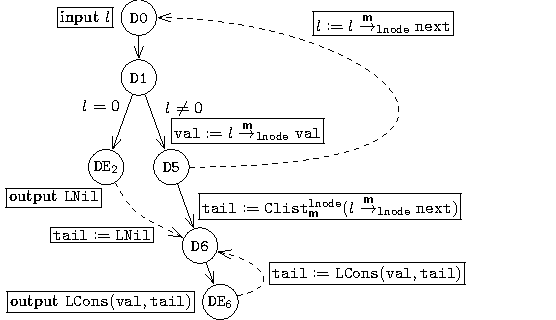
\includegraphics[scale=1]{chapters/figures/figClistDeconsCfg.pdf}
\end{center}
\vspace{5px}
\caption{\label{fig:clistdeconsCFG}CFG of Deconstruction Program}
\end{subfigure}%
\\
\end{tabular}
\caption{\label{fig:clistdecons}IR and CFG representation of deconstruction program based on the lifting constructor \lift{list}{}{lnode} defined in \cref{eqn:clist}.
In \cref{fig:clistdeconsIR}, \dpc{6} contains a recursive function call. In \cref{fig:clistdeconsCFG}, the square boxes show the transfer functions for the deconstruction program.
The dashed edges represent the recursive function call in the CFG representation as shown in \cref{fig:clistdeconsCFG}.}
\end{figure}

\begin{theorem}
\label{theorem:clistsEqual}
Under an antecedent \lhs{},
$\lifted{list}{\mem{}}{lnode}{\cv{l}} \indEq{} \lifted{list}{\mem{}'}{lnode}{\cv{l}}$ holds
{\em if and only if} the two deconstruction programs $\dprog{}_1$ and $\dprog{}_2$, based on \lifted{list}{\mem{}}{lnode}{\cv{l}}
and \lifted{list}{\mem{}'}{lnode}{\cv{l}}, are equivalent.
The equivalence must ensure that the observables generated by both programs
(i.e. output \type{List} values) are equal, given the that input $\cv{l}$
is provided to both programs respectively {\em and}
the antecedent \lhs{} holds at the program entries.
\end{theorem}
\begin{proofsketch}
The proof follows from noting that the only observables of $\dprog{}_1$ and $\dprog{}_2$ are their output \type{List} values.
Also, the value represented by a lifted expression is equal to the output of its deconstruction program.
Thus, a successful equivalence proof ensures equal values represented by the lifting constructors and vice versa.
\end{proofsketch}

Thus, to check if $\lifted{list}{\mem{}}{lnode}{\cv{l}} \indEq{} \lifted{list}{\mem{}'}{lnode}{\cv{l}}$
holds; we instead check if a bisimulation relation exists between their respective
deconstruction programs \fdprog{} and \sdprog{} (implying equivalence).
\Cref{theorem:clistsEqual} generalizes to arbitrary lifted expressions
with potentially different \cprog{} values and memory states.

\begin{figure}[H]
\begin{tabular}{@{}c@{}c@{}}
\begin{subfigure}[b]{0.4\textwidth}
\begin{center}
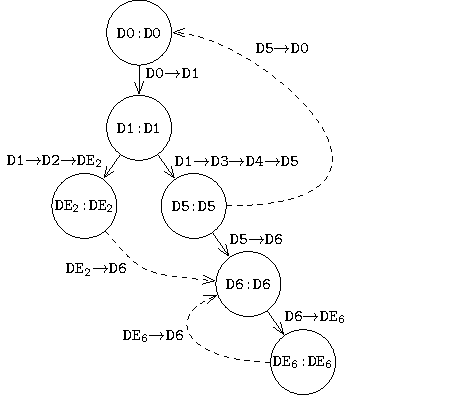
\includegraphics[scale=1]{chapters/figures/figClistDeconsProductCfg.pdf}
\end{center}
\caption{\label{fig:clistdeconsproductcfg} Decons-PCFG}
\end{subfigure}%
&
\begin{subfigure}[b]{0.6\textwidth}
\begin{center}
\begin{footnotesize}
\renewcommand{\arraystretch}{1.6}
\begin{tabular}{|c|l|}
\hline
{\bf PC-Pair} & \multicolumn{1}{c|}{\bf Invariants} \\
\hline
\hline
(\ddpc{0}{0}) & \Tstrut $\circled{\small P} \  \fstv{l} = \sndv{l}$ \\
\hline
(\ddpc{1}{1}) & \Tstrut $\circled{I1} \  \fstv{l} = \sndv{l}$ \\
\hline
\multirow{2}{*}{(\ddpc{5}{5})} &
\Tstrut $\circled{I2} \  \fstv{val} = \sndv{val}$ \\
& \Bstrut $\circled{I3} \  \structPointer{\fstv{l}}{\mem{}}{lnode}{next} = \structPointer{\sndv{l}}{\mem{}'}{lnode}{next}$ \\
\hline
\multirow{2}{*}{(\ddpc{6}{6})} &
\Tstrut $\circled{I4} \  \fstv{val} = \sndv{val}$ \\
& \Tstrut \Bstrut $\circled{I5} \  \fstv{tail} = \sndv{tail}$ \\
\hline
\Tstrut (\ddpc{E_2}{E_2}) &
\multirow{2}{*}{$\circled{E} \   \fstv{ret} = \sndv{ret}$} \\
\Bstrut (\ddpc{E_6}{E_6}) & \\
\hline
\end{tabular}
\end{footnotesize}
\end{center}
\caption{\label{fig:clistdeconsproductcfginvs} Invariants Table}
\end{subfigure}%
\\
\end{tabular}
\caption{\label{fig:clistdeconsproductcfgandinvs} Decons-PCFG and invariants table for the deconstruction programs of \lifted{list}{\mem{}}{lnode}{\cv{l}} and \lifted{list}{\mem{}'}{lnode}{\cv{l}} respectively.}
\end{figure}

\subsubsection{Checking Bisimulation between Deconstruction Programs}
\label{sec:reconsbisim}
To check bisimulation, we attempt to show that both deconstructions
proceed in lockstep, and the invariants at each step of this lockstep execution ensure equal observables.
We use a product-CFG to encode this lockstep execution between \fdprog{} and \sdprog{} ---
to distinguish this product-CFG from the top-level product-CFG that relates \sprog{} and \cprog{},
we call this product-CFG that relates two deconstruction programs,
a {\em deconstruction product}-CFG or {\em decons}-PCFG for short.

The decons-PCFG for the proof obligation in \cref{eqn:clistPreserved} is shown in \cref{fig:clistdeconsproductcfg}.
We distinguish states between the first and second programs using superscripts:
$fst$ and $snd$ respectively.
However, these are omitted in case the states are equal in both programs (e.g., \cv{p}).
To check bisimulation between the programs that deconstruct
\lifted{list}{\mem{}}{lnode}{\cv{l}} and \lifted{list}{\mem{}'}{lnode}{\cv{l}} (i.e. \fdprog{} and \sdprog{} respectively),
the decons-PCFG correlates one unrolling of the first program with one unrolling
of the second program, as defined by the unrolling procedure in \cref{eqn:clist}.
Thus, the PC-transition correlations of \fdprog{} and \sdprog{} are trivially
obtained by unifying the static program structures as shown in \cref{fig:clistdeconsproductcfg}.
A node is created in the decons-PCFG that encodes the correlation of the entries
of both programs; we call this node the {\em recursive-node} in the decons-PCFG (e.g., (\ddpc{0}{0}) in \cref{fig:clistdeconsproductcfg}).
A recursive call becomes a back-edge in the decons-PCFG that terminates at the recursive-node.
Furthermore, a bisimulation check involves identification of invariants at correlated PC-pairs strong enough to
ensure observable equivalence.
At the start of both deconstruction programs, \circled{\small P} $\fstv{l} = \sndv{l} = \cv{l}$ --- the same \cv{l}
is passed to both \fdprog{} and \sdprog{}, only the memory states $\mem{}$
and $\mem{}'$ (defined in \cref{eqn:memstore}) are different.
The observables include the returned \type{List} values at correlated
program exits (\ddpc{E_2}{E_2}) and (\ddpc{E_6}{E_6}),
which forms the postcondition (labeled \circled{\small E} in \cref{fig:clistdeconsproductcfginvs}).
Next, the bisimulation check involves identification of inductive invariants (labeled \circled{\small I}
in \cref{fig:clistdeconsproductcfginvs}) at correlated PC-pairs.
The proof obligations arising due to this bisimulation check include:

\begin{enumerate}
\item The \underline{\tt if} condition $(\fstv{l} = 0)$ in \fdprog{} is equal to the corresponding \underline{\tt if} condition $(\sndv{l} = 0)$ in \sdprog{}:
$(\fstv{l} = 0) = (\sndv{l} = 0)$.
\item If the \underline{\tt if} condition evaluates to false in both \fdprog{} and \sdprog{},
then observable values \fstv{val} and \sndv{val} along the path \ddedge{1}{1}{5}{5}
(used in the construction of the output lists) are equal.
This forms the invariant \circled{\small I2} in \cref{fig:clistdeconsproductcfginvs} and lowers to the following proof obligation: \\
$(\fstv{l} \neq 0) \land (\sndv{l} \neq 0) \Rightarrow \structPointer{\fstv{l}}{\mem{}}{lnode}{val} = \structPointer{\sndv{l}}{\mem{}'}{lnode}{val}$.
\item If the \underline{\tt if} condition evaluates to false in both \fdprog{} and \sdprog{}, then the
preconditions are satisfied at the beginning of the programs invoked through the recursive call.
This involves checking that, along the path \ddedge{1}{1}{5}{5}, the actual arguments to the recursive call
satisfies the precondition \circled{\small P}
at the beginning of the procedure i.e. the recursive-node (\ddpc{0}{0}).
This forms the invariant \circled{\small I3} in \cref{fig:clistdeconsproductcfginvs} and lowers the following proof obligation: \\
$(\fstv{l} \neq 0) \land (\sndv{l} \neq 0) \Rightarrow \structPointer{\fstv{l}}{\mem{}}{lnode}{next} = \structPointer{\sndv{l}}{\mem{}'}{lnode}{next}$.

A successful discharge of the above invariant (\circled{\small I3}), by induction, ensures that postcondition (\circled{E})
is satisfied by the values returned by the recursive call at product-CFG node (\ddpc{6}{6}).
Hence, we can assume that invariant \circled{\small I5} holds at (\ddpc{6}{6}).
This special case of correlating procedure call edges is further discussed in \cref{sec:correlfcalls} as part of our
overall product-CFG construction algorithm.
\end{enumerate}

The first check succeeds due to the precondition \circled{\small P} $\fstv{l} = \sndv{l}$ at the recursive-node.
For the second and third checks, we additionally need to reason that the memory objects
$\structPointer{\sndv{l}}{\mem{}'}{lnode}{val}$ and
$\structPointer{\sndv{l}}{\mem{}'}{lnode}{next}$ cannot alias with
the writes in $\mem{}'$ (\cref{eqn:memstore}) to the newly
allocated objects
$\structPointer{\cv{p}}{\mem{}'}{lnode}{val}$ and
$\structPointer{\cv{p}}{\mem{}'}{lnode}{next}$.
We capture this aliasing information using a points-to analysis described next in \cref{sec:pointsTo}.

Notice that a bisimulation check between the deconstruction programs is
significantly easier than the top-level bisimulation check between \sprog{} and \cprog{}:
here, the correlation of PC traisitons is trivially identified by unifying the
unrolling procedures of both lifted expressions, and the candidate invariants
are obtained by equating each pair of terminal values that form the observables
of both programs.

\subsubsection{Points-to Analysis}
\label{sec:pointsTo}
To reason about aliasing (as required during bisimulation check in \cref{sec:bisim}),
we conservatively compute {\em may-point-to} information for each program value using
an interprocedural flow-sensitive version of Andersen's algorithm \cite{andersen94programanalysis}.
The range of this computed may-point-to function is the set of {\em region labels},
where each region label identifies a set of memory objects.
The sets of memory objects identified by two distinct region labels
are necessarily disjoint.
We write $p \pointsTo{} \{ \mlr{R_1}, \mlr{R_2} \}$ to represent the condition that value $p$
{\em may point to} an object belonging to one of the region labels \mlr{R_1} or \mlr{R_2}
(but may not point to any object outside of \mlr{R_1} and \mlr{R_2}).

We populate the set of all region labels using {\em allocation sites} of the \cprog{} program
i.e., PCs where a call to {\tt malloc} occurs.
For example, \cpc{4} in \cref{fig:llAllocCIR} is an allocation site.
For each allocation site $A$, we create two region labels:
(a) the first region label, called $A_1$, identifies the set of memory objects
that were allocated by the most recent execution of $A$, and (b) the second region
label, called $A_{2+}$, identifies the set of memory objects that were allocated
by older (not the most recent) executions of $A$.
We also include a special heap region, $\mathcal{H}$ to represent
the rest of the memory not covered by the allocation site regions.

For example, at the start of PC \cpc{7} in \cref{fig:llAllocCIR},
$\cv{i} \pointsTo{} \emptyset$, $\cv{p} \pointsTo{} \{ \mlrf{\cpc{4}} \}$,
and $\cv{l} \pointsTo{} \{ \mlrs{\cpc{4}} \}$.
Since the may-point-to analysis determines the sets of objects pointed-to
by \cv{p} and \cv{l} to be disjoint, (\mlrf{\cpc{4}} against \mlrs{\cpc{4}}),
any memory accessed through \cv{p} and \cv{l} cannot alias at \cpc{7}
(for accesses within the bounds of the allocated objects).

The may-point-to information is computed not just for program values (e.g., \cv{p}, \cv{l})
but also for each region label.
For region labels \mlr{R1}, \mlr{R2} and \mlr{R3}:
$\mlr{R1} \pointsTo{} \{ \mlr{R2}, \mlr{R3} \}$ represents the condition that
the values (pointers) stored in objects identified by \mlr{R1} may point to objects
identified by either \mlr{R2} or \mlr{R3} (but not to any other object outside \mlr{R2} and \mlr{R3}).
In \cref{fig:llAllocCIR}, at PC \cpc{7}, we get
$\mlrf{\cpc{4}} \pointsTo{} \{ \mlrs{\cpc{4}} \}$ and
$\mlrs{\cpc{4}} \pointsTo{} \{ \mlrs{\cpc{4}}, \mathcal{H} \}$.
The condition $\mlrf{\cpc{4}} \pointsTo{} \{ \mlrs{\cpc{4}} \}$ holds
because the \field{next} pointer of the object pointed-to by \cv{p}
(which is a \mlrf{C4} object at \cpc{7}) may point to a \mlrs{\cpc{4}}
object (e.g., object pointed to by \cv{l}).
On the other hand, pointers within a \mlrs{\cpc{4}} object may not point to a \mlrf{\cpc{4}} object.

\begin{figure}
\begin{tabular}{@{}c@{}c@{}}
\begin{subfigure}[b]{0.5\textwidth}
\begin{center}
\begin{footnotesize}
\renewcommand{\arraystretch}{1.6}
\begin{tabular}{|ll|}
\hline
\multicolumn{2}{|c|}{\bf Points-to Invariants} \\
\hline
\hline
$\circled{\footnotesize J1} \  \cv{p} \pointsTo{} \{ \mlrf{\cpc{4}} \}$ & $\circled{\footnotesize J2} \  \mlrf{\cpc{4}} \pointsTo{} \{ \mlrs{\cpc{4}} \}$ \\
$\circled{\footnotesize J3} \  \cv{l} \pointsTo{} \{ \mlrs{\cpc{4}} \}$ & $\circled{\footnotesize J4} \  \mlrs{\cpc{4}} \pointsTo{} \{ \mlrs{\cpc{4}}, \heapr{} \}$ \\
$\circled{\footnotesize J5} \  \cv{i} \pointsTo{} \emptyset$            & $\circled{\footnotesize J6} \  \heapr{} \pointsTo{} \{ \mlrs{\cpc{4}}, \heapr{} \}$ \\
\hline
\end{tabular}
\end{footnotesize}
\end{center}
\caption{\label{fig:clistdeconspointstoinvs} Points-to Invariants at \cpc{5} of \cref{fig:llAllocCIR}}
\end{subfigure}%
&
\begin{subfigure}[b]{0.5\textwidth}
\begin{center}
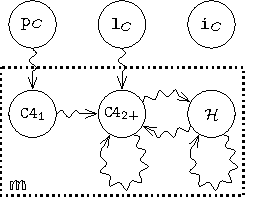
\includegraphics[scale=1]{chapters/figures/figClistDeconsCfgPointstoGraph.pdf}
\end{center}
\caption{\label{fig:clistdeconspointstograph} Points-to Graph at \cpc{5} of \cref{fig:llAllocCIR}}
\end{subfigure}%
\\
\end{tabular}
\caption{\label{fig:clistdeconspointstoinvsandgraph} Points-to Invariants and Points-to Graph at \cpc{5} of \cref{fig:llAllocCIR}}
\end{figure}

\subsubsection{Transferring Points-to Information to Decons-PCFG}
\label{sec:pointsToAsInvariants}
Recall that in \cref{sec:reconsbisim}, we reduce the condition
$\lifted{list}{\mem{}}{lnode}{\cv{l}} \indEq{} \lifted{list}{\mem{}'}{lnode}{\cv{l}}$
to an equivalence check between their deconstruction programs: \fdprog{} and \sdprog{}.
Also, recall that we discharge the equivalence check through construction of a
decons-PCFG encoding the lockstep execution of the two deconstruction programs.
During this bisimulation check, we need to prove that,
$\structPointer{\fstv{l}}{\mem{}}{lnode}{\{val,next\}}$ and
$\structPointer{\sndv{l}}{\mem{}'}{lnode}{\{val,next\}}$ are equal.
Recall that the invariant \circled{\small I1} (in \cref{fig:clistdeconsproductcfginvs})
asserts $\fstv{l} = \sndv{l} (\triangleq \comv{l})$.
Thus, to successfully discharge these proof obligations, it suffices to show that \comv{l}
cannot alias with the memory writes that distinguish \mem{} and $\mem{}'$.

\Cref{fig:clistdeconspointstoinvs} shows the may-point-to relations identified by our
points-to analysis on the \cprog{} in \cref{fig:llAllocCIR} at the program point \cpc{5}.
The points-to analysis determines that at \cpc{5}
(i.e. start of the product-CFG edge \scedge{3}{5}{3}{3} across which the proof obligation
is generated), the pointer to the {\em head} of the list, i.e. \circled{\small J3} $\cv{l} \pointsTo{} \{ \mlrs{C4} \}$.
It also determines that the distinguishing writes (in \cref{eqn:memstore}) modify memory regions
belonging to \mlrf{C4} only (i.e. \circled{\small J1}).
Further, we get \circled{\small J4} $\mlrs{C4} \pointsTo{} \{ \mlrs{C4}, \heapr{} \}$ at PC \cpc{5}.
\Cref{fig:clistdeconspointstograph} shows the points-to graph for the \cprog{} variables and the memory regions (in \mem{}).
This graphical representation clearly illustrates that the objects pointed to by \cv{p} (i.e. \mlrf{\cpc{4}})
and \cv{l} (i.e. \mlrs{\cpc{4}}) are mutually isolated.

However, notice that these determinations only rule out aliasing of the list-head with
the distinguishing writes. We also need to confirm non-aliasing
of the internal nodes of the linked list with the distinguishing writes.
For this, we need to identify a points-to invariant: $\sndv{l} \pointsTo{} \{ \mlrs{C4}, \heapr{} \}$,
at the recursive-node of the decons-PCFG (shown in \cref{fig:clistdeconsproductcfg}).
To identify such points-to invariants, we run our points-to analysis
on the deconstruction programs (i.e. \fdprog{} and \sdprog{}) before comparing them for equivalence.
To model procedure calls, A {\em supergraph} is created with edges representing control flow
to (and from) the entry (and exits) of the program respectively (e.g., dashes edges in \cref{fig:clistdeconsCFG}).
To see why $\sndv{l} \pointsTo{} \{ \mlrs{C4}, \heapr{} \}$ is an inductive invariant at (\ddpc{0}{0}):

\begin{itemize}
\item[] (Base case) the invariant holds at entry of the decons-PCFG because \sndv{l} = \cv{l} at entry
and \circled{\small J3} $\cv{l} \pointsTo{} \{ \mlrs{C4} \}$, which is a stronger condition.
\item[] (Inductive step) if $\sndv{l} \pointsTo{} \{ \mlrs{C4}, \heapr{} \}$ holds at the entry node,
it also holds at the start of a recursive call.
This follows from \circled{\small J4} $\mlrs{C4} \pointsTo{} \{ \mlrs{C4}, \heapr{} \}$
and \circled{\small J5} $\heapr{} \pointsTo{} \{ \mlrs{C4}, \heapr{} \}$ (points-to information at PC \cpc{5}),
which ensures that $\structPointer{\cv{l}}{\mem{}'}{lnode}{next}$ may point to only \mlrs{C4} and \heapr{} objects.
\end{itemize}

The same analysis is run for both \cprog{}, and the deconstruction programs \fdprog{} and \sdprog{}.
For a deconstruction program \dprog{}, the boundary condition (at entry) for the
points-to analysis is based on the results of the points-to analysis on \cprog{}
at the PC where the proof obligation is being discharged.
For example, the points-to information of \cprog{} PC \cpc{5} (in \cref{fig:llAllocCIR})
is used during the points-to analysis on \fdprog{} and \sdprog{}.

During proof query discharge, the points-to invariants are encoded as SMT constraints.
This allows us to complete the bisimulation proof on the decons-PCFG in \cref{fig:clistdeconsproductcfg},
and consequently, successfully discharge the proof obligation
\hoareTriple{\scpcinv{3}{5}}{\spath{3,5,3},\cpath{5,3}}{\sv{l} \indEq{} \lifted{list}{\mem{}}{lnode}{\cv{l}}}
in \cref{tab:llproductInv}.
The points-to analysis is further discussed in \cref{sec:pointsToFormal}.

\subsubsection{Summary of Type III Proof Discharge Algorithm}
\label{sec:cat3summary}

Before the start of an equivalence check, a points-to analysis is run on the \cprog{} program (IR) once.
During equivalence check, to discharge a type III proof obligation $P: \lhs{} \Rightarrow \rhs{}$
(expressed first-order logic), we substitute ADT values (in \sprog{}) in the \rhs{} with
lifted C values (in \cprog{}), based on the \recursiveRelations{} present in the \lhs{}.
This is followed by decomposition of \rhs{} and \rhs{}-breaking.

Upon \rhs{}-breaking, we obtain several smaller proof obligations,
say $P_i : \lhs{}_i \Rightarrow \rhs{}_i$ (for $i=1\ldots n$).
To prove $P$, we require {\em all} of these smaller proof obligations $P_i$ to be provable.
However, a counterexample to {\em any} one of these proof obligations would also be
a counterexample to the original proof obligation $P$.
Due to decomposition and \rhs{}-breaking, each $\rhs{}_i$ must be a decomposition clause
and hence, relate atomic expressions.
If $\rhs{}_i$ relate two scalar values, then $P_i$ is a type II proof obligation and
discharged using the algorithm summarized in \cref{sec:cat2summary}.

If $\rhs{}_i$ relates two lifted expressions (i.e. a \recursiveRelation{}),
we check if the deconstruction programs of the two ADT values being compared
can be proven to be equivalent (assuming $\lhs{}_i$ holds at the correlated entry nodes
on the first invocation).
Similar to the top-level equivalence check, we attempt to find a bisimulation relation.
To improve the precision during bisimilarity check, we transfer points-to invariants of the \cprog{}
program (at the PC where the proof obligation is being discharged) to the entry of the
deconstruction programs. The same points-to analysis is run on the deconstruction
programs before the equivalence check begins, (through construction of decons-PCFG)
to identify points-to invariants in the deconstruction programs.

If the bisimilarity check succeeds, we return {\em true} for $P$;
otherwise, we imprecisely return {\em false} (without counterexamples).

\begin{figure}
\begin{algorithm}[H]
\begin{footnotesize}
\DontPrintSemicolon
\everypar={\nl}
\SetAlgoLined
\SetKwProg{Fn}{Function}{}{end}
\Fn{$prove(\hoareTriple{\phi_s}{\rho_S,\rho_C}{\phi_d}, k, d_o, d_u)$}{
  $F \mapsfrom {\tt lowerWP}(\hoareTriple{\phi_s}{\rho_S,\rho_C}{\phi_d})$\\
  \ForEach{$\lhs{} \Rightarrow \rhs{}_i \keyword{in} {\tt RHSBreak}(F)$}{
    \If{$solve(\lhs{}, \rhs{}_i, k, d_o, d_u) = \cons{False}(\Gamma)$}{
      \Return{$\cons{False}(\Gamma)$}
    }
  }
  \Return{$\cons{True}$}
}
\Fn{$solve(\lhs{}, \rhs{}, k, d_o, d_u)$}{
  $(\lhs{}_k, \rhs{}_k) \mapsfrom {\tt decomposeAndUnroll}(\lhs{}, \rhs{}, k)$\\
  \Switch{${\tt categorize}(\lhs{}_k, \rhs{}_k)$}{
    \uCase{${\tt Type\ I}$}{
      \Return{${\tt solveSMT}(\lhs{}_k \Rightarrow \rhs{}_k)$}
    }
    \uCase{${\tt Type\ II}$}{
      $\lhs{}_o \mapsfrom {\tt overapproximate}(\lhs{}, d_o)$\\
      \If{${\tt solveSMT}(\lhs{}_o \Rightarrow \rhs{}_k) = \cons{True}$}{
        \Return{$\cons{True}$}
      }
      $\lhs{}_u \mapsfrom {\tt underapproximate}(\lhs{}, d_u)$\\
      \If{${\tt solveSMT}(\lhs{}_u \Rightarrow \rhs{}_k) = \cons{False}(\Gamma)$}{
        \Return{$\cons{False}(\Gamma)$}
      }
      \Return{$\cons{False}(\emptyset)$}
    }
    \Case{${\tt Type\ III}$}{
      $\rhs{}' \mapsfrom {\tt rewriteRHSUsingLHS}(\lhs{}, \rhs{})$\\
      \ForEach{${\tt P}_i \Rightarrow \rhs{}_i \keyword{in} {\tt decompose}(\rhs{}')$}{
        \uIf{$\rhs{}_i = l_1\indEq{}l_2$}{
          $(\dprog{}_1,\dprog{}_2) \mapsfrom {\tt getDeconstructionPrograms}(l_1,l_2)$\\
          \If{${\tt checkEquivalence}(\lhs{} \land {\tt P}_i,\dprog{}_1,\dprog{}_2) = \cons{False}$}{
            \Return{$\cons{False}(\emptyset)$}
          }
        }
        \ElseIf{$solve(\lhs{} \land {\tt P}_i, \rhs{}_i, k, d_o, d_u) = \cons{False}(\Gamma)$}{
          \Return{$\cons{False}(\Gamma)$}
        }
      }
      \Return{$\cons{True}$}
    }
  }
}
\end{footnotesize}
\caption{Algorithm for discharging proof obligations containing \recursiveRelations{}}
\end{algorithm}
\caption{\label{algo:proofSummary}Pseudocode of the algorithm responsible for discharging proof obligations containing \recursiveRelations{}.}
\end{figure}

\subsection{Overview of Proof Discharge Algorithm}
\Cref{algo:proofSummary} gives a basic pseudo-code of our proof discharge algorithm.
The top-level function responsible for discharging Hoare triple proof obligations is: $Prove()$.
$Prove()$ accepts the proof obligation along with the categorization ($k$)
and approximation ($d_o$ and $d_u$) parameters.
$Prove()$ either returns \cons{True} representing a successful proof attempt,
or it returns \cons{False}($\Gamma$), where $\Gamma$ is a set of counterexamples.
Recall that our proof discharge algortihm is {\em sound} and may return \cons{False}($\emptyset$)
to indicate a failed (proof and counterexample generation) attempt.
As discussed in \cref{sec:proofobl}, we lower the Hoare triple into a first-order logic
formula ($F$) using weakest-precondition predicate transformer.
This is followed by \rhs{}-breaking (introduced in \cref{sec:proofalgoprops}),
which results in multiple smaller proof obligations.
$Prove{}$ attempts to prove each of these proof obligations individually through a call to $Solve()$.
If any one of these queries fail, we immediately stop and return \cons{False} with the
counterexamples in $\Gamma$ --- a counterexample to one of the smaller queries is also a counterexample
to the original query.

$Solve()$ is responsible for discharging these smaller queries.
Inputs include \lhs{}, \rhs{} (representing the proof obligation $P :\lhs{} \Rightarrow \rhs{}$);
along with the parameters: $k$, $d_o$ and $d_u$.
$Solve()$ begins by finding the $k$-unrolled form of $P$ and categorizes it into one of the three types.
As discussed in \cref{sec:cat1}, we simply discharge a type I query using SMT solvers (through $SMTProve()$).
$SMTProve()$ is responsible for (a) translating the input formula (absent of \recursiveRelations{})
to SMT logic, and (b) reconstruction of counterexamples from the models returned by the SMT solvers.
These two topics are further explored in \cref{sec:smtencoding,sec:cerecons} respectively.
As summarized in \cref{sec:cat2summary}, for a type II query, we attempt to prove its
overapproximate version first.
In case of a failure, we attempt to disprove (and generate counterexamples) its underapproximate version.
If both attempts fail, we {\em soundly} return \cons{False} (without counterexamples).
Lastly, a type III query $P$ is discharged as detailed in \cref{sec:cat3summary}.
In brief, we decompose and perform \rhs{}-breaking on $P$.
This results in smaller proof obligations; ones without a \recursiveRelation{} in its \rhs{},
are type II queries and discharged through a recursive call to $Solve()$.
For those containing a \recursiveRelation{} $l_1 \indEq{} l_2$ in their \rhs{}, we reformulate the query as an
equivalence check between the deconstruction program of $l_1$ and $l_2$ respectively.
If any one of these queries fail, we immediately return \cons{False} with the counterexamples (if available).
Otherwise, we have successfully proven a type III query and return \cons{True}.
